% SC3099 — Chapter 2: Requirements Engineering (0->100 ground-up)
\chapter{Requirements Engineering}\label{ch:requirements}

\begin{quote}
\emph{``Building the wrong thing, perfectly, is still failure.''} Requirements say \emph{what} the system must do before we decide \emph{how} to build it. Get them wrong and every later diagram, line of code, and test answers the wrong question.
\end{quote}

\noindent\fbox{\parbox{\dimexpr\linewidth-2\fboxsep-2\fboxrule}{%
\textbf{From zero: no prior RE knowledge assumed.} We start with people who care, then ask how to listen to them, how to write down what they need without ambiguity, how to choose what matters most, and how to prove every need is met. No UML, agile, or modelling assumed.}}
\vspace{0.4em}

\section*{Learning Outcomes}
After this chapter you will be able to:
\begin{enumerate}[label=(L\arabic*)]
    \item identify stakeholders and position them on a power--interest grid;
    \item select and apply elicitation techniques suited to the project context;
    \item distinguish functional vs.\ non-functional requirements and write INVEST user stories and use cases;
    \item prioritise a backlog using MoSCoW and justify trade-offs;
    \item validate requirements and construct a traceability matrix from needs to tests.
\end{enumerate}
In this chapter we follow a single running example (campus food delivery) so each technique can be compared on the same problem. Replace it with your capstone domain as you read.
We assume no prior exposure to RE; intuition precedes formalism throughout.

% ============================================================
\section{Stakeholders: Who Wants What?}
\label{sec:stakeholders}
A \emph{stakeholder} is anyone who affects or is affected by the system: users, sponsors, operators, regulators, maintainers, even adversaries. Missing one means missing requirements. For a campus food-delivery app, stakeholders include students (end users), hawkers (suppliers), the university (sponsor), the delivery riders, the payment gateway, and the Personal Data Protection Commission (regulator). Their goals conflict --- students want speed, hawkers want accuracy, finance wants auditability.

The \textbf{power--interest grid} maps influence (can they stop the project?) against concern (do they care daily?). Each quadrant demands a different strategy.

\begin{figure}[h]
\centering
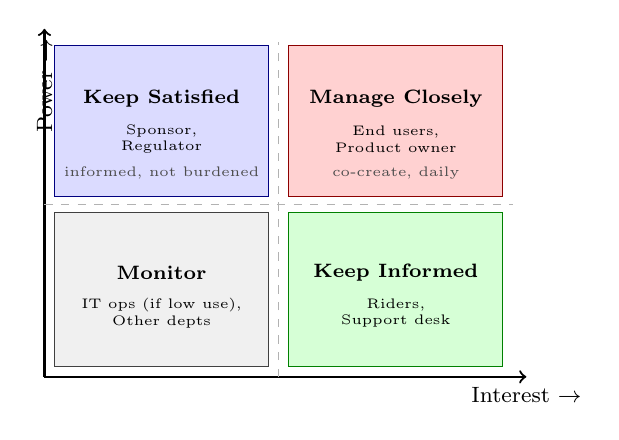
\begin{tikzpicture}[scale=0.85, every node/.style={font=\scriptsize}]
% axes
\draw[->, thick] (0,0) -- (7.2,0) node[below, font=\footnotesize] {Interest $\rightarrow$};
\draw[->, thick] (0,0) -- (0,5.2) node[left, font=\footnotesize, rotate=90] {Power $\rightarrow$};
% 4 quadrants with fills
\fill[blue!14, draw=blue!50!black] (0.15,2.7) rectangle (3.35,4.95);
\fill[red!18, draw=red!55!black] (3.65,2.7) rectangle (6.85,4.95);
\fill[gray!12, draw=gray!50!black] (0.15,0.15) rectangle (3.35,2.45);
\fill[green!16, draw=green!50!black] (3.65,0.15) rectangle (6.85,2.45);
% labels inside
\node[align=center, font=\scriptsize\bfseries] at (1.75,4.15) {Keep Satisfied};
\node[align=center, font=\tiny] at (1.75,3.55) {Sponsor,\\Regulator};
\node[align=center, font=\tiny, text=gray!60!black] at (1.75,3.05) {informed, not burdened};
\node[align=center, font=\scriptsize\bfseries] at (5.25,4.15) {Manage Closely};
\node[align=center, font=\tiny] at (5.25,3.55) {End users,\\Product owner};
\node[align=center, font=\tiny, text=gray!60!black] at (5.25,3.05) {co-create, daily};
\node[align=center, font=\scriptsize\bfseries] at (1.75,1.55) {Monitor};
\node[align=center, font=\tiny] at (1.75,0.95) {IT ops (if low use),\\Other depts};
\node[align=center, font=\scriptsize\bfseries] at (5.25,1.55) {Keep Informed};
\node[align=center, font=\tiny] at (5.25,0.95) {Riders,\\Support desk};
% quadrant boundary lines emphasized
\draw[dashed, gray!60] (3.5,0) -- (3.5,5.0);
\draw[dashed, gray!60] (0,2.58) -- (7.0,2.58);
\end{tikzpicture}
\caption{Power--interest grid: four stakeholder strategies. Colour guides attention --- red needs most effort. Place every named stakeholder; empty quadrants signal missed people.}
\label{fig:power-interest}
\end{figure}

A useful lens is the \emph{stakeholder onion}: core (hands on keyboard), containing (organisation that owns the system), and surrounding (society, regulators). Walk outward layer by layer so hidden stakeholders surface. Conflicts are normal: rank by power and urgency, negotiate trade-offs in workshops, and record rationale so later changes have context.

Identify by brainstorming roles, snowballing (``who else?'') and checking organisational charts, then place. Revisit every sprint: power and interest shift as the system becomes real. A sponsor who was low-interest at kickoff may become high-interest when money is spent; a regulator may gain power when a new PDPA guideline appears. Tracking movement on the grid is an early warning system.

For each stakeholder also note their \emph{success criterion}: what would make them declare the project a success? Students say ``food in 15\,min''; hawkers say ``zero wrong orders''; finance says ``every dollar reconciled''. Conflicting criteria become trade-offs for MoSCoW.

% ============================================================
\section{Elicitation Techniques}
\label{sec:elicitation}
Elicitation is structured listening. No single method finds all requirements, so triangulate.

\begin{itemize}[leftmargin=*]
    \item \textbf{Interviews} (1--1, semi-structured). Best for depth, sensitive topics, and expert tacit knowledge. Prepare open questions, follow up with ``why?'', record word-for-word notes. Cost: time; risk: interviewer bias.
    \item \textbf{Workshops} (facilitated group). Best for consensus and conflict resolution among competing stakeholders. Use brainstorming, card sorting, or story mapping. Needs skilled facilitation to avoid loud-voice wins.
    \item \textbf{Observation.} Best when users cannot
    articulate workflow (they have normalised workarounds).
    Shadow riders on delivery runs; note deviations from the
    ``official'' process. Reveals real, not imagined, tasks.
    \item \textbf{Questionnaires / surveys.} Best for breadth across many users. Closed questions quantify; open questions surprise. Cheap to distribute, but poor for probing. Pilot first --- ambiguous wording destroys data.
\end{itemize}

Triangulate: use at least two methods per major requirement. For the food app, interview two hawkers, observe lunch rush for two days, then survey 80 students to confirm frequency. Cross-check what people say versus what they do. Respect ethics: inform participants, anonymise data, and obtain consent before recording --- especially under PDPA.

Choose by risk: safety-critical flows need observation plus interviews; broad preference data suits surveys; early scoping suits workshops. Document each finding as a candidate requirement with ID, source, and priority so nothing evaporates after the meeting.

Workshops benefit from a neutral facilitator and time-boxed agenda: diverge (generate), then converge (cluster and vote). Capture decisions on a visible board; photograph it. Without a written record, consensus evaporates by the next day. Always record source, date, and rationale for each requirement that emerges --- this seeds traceability.

% ============================================================
\section{Specification: Saying It Precisely}
\label{sec:specification}
Raw stakeholder wishes are ambiguous. A \emph{specification} turns them into testable statements.

\paragraph{Functional vs.\ non-functional (NFR).} Functional (FR): \emph{what} the system does --- ``a student can cancel an order before acceptance.'' NFR: \emph{how well} --- performance (p95 latency $<2$\,s), security (TLS\,1.3, PDPA), usability (WCAG\,2.1 AA), reliability (99.5\% uptime), constraints (runs on Android 10+). NFRs need quantification; ``fast'' is not a requirement, ``$<2$\,s at 1000 concurrent users'' is.

\paragraph{User stories and INVEST.} Agile teams capture FRs as stories: \emph{As a $\langle$role$\rangle$ I want $\langle$goal$\rangle$ so that $\langle$benefit$\rangle$.} The INVEST checklist tests story quality: \textbf{I}ndependent, \textbf{N}egotiable, \textbf{V}aluable, \textbf{E}stimable, \textbf{S}mall, \textbf{T}estable. A story that cannot be tested is a wish, not a requirement.

NFRs are measured: response time at a load, throughput (orders/min), learnability (time to first order $<3$\,min), and availability ($99.5\%$ $\approx 3.6$\,h downtime/month). Each NFR needs metric, target, and test method or it will be ignored in implementation.
For example, ``usability'' becomes ``a new student completes first order in $<3$\,min without help (measured in usability test with 5 participants)'', and ``reliability'' becomes ``order service uptime $\ge 99.5\%$ measured monthly via synthetic probes''.

\paragraph{Use cases.} A use case details the interaction between actors and system to achieve a goal, including main success path and extensions (errors, alternates). Use cases are richer than stories and suit regulated or complex flows.

\begin{lstlisting}[language=Python, caption={User story with Gherkin acceptance criteria --- executable specification}, label={lst:user-story}]
# User Story US-07
# As a student, I want to cancel my order before the hawker accepts
# so that I am not charged for a mistake.

Feature: Order cancellation

  Scenario: Cancel before acceptance
    Given order "ORD-42" is in state "PENDING"
    And the current user is the order owner
    When the user cancels order "ORD-42"
    Then the order state becomes "CANCELLED"
    And no payment is captured
    And the hawker receives a "CANCELLED" notification

  Scenario: Cancel after acceptance is rejected
    Given order "ORD-42" is in state "ACCEPTED"
    When the user cancels order "ORD-42"
    Then the system returns error "Too late to cancel"
    And the order state remains "ACCEPTED"
\end{lstlisting}

Each story gets an ID (US-07) and priority (MoSCoW). The ID links forward to design and tests, enabling the traceability matrix in~\S\ref{sec:validation}.

Gherkin makes the story \emph{testable}: each Then is an assertion; the whole scenario runs as an automated acceptance test. Link story ID US-07 to later design, code, and tests.

% ============================================================
\section{MoSCoW Prioritisation}
\label{sec:moscow}
Not everything can ship at once. MoSCoW forces honest trade-offs under fixed time and people.

\begin{figure}[h]
\centering
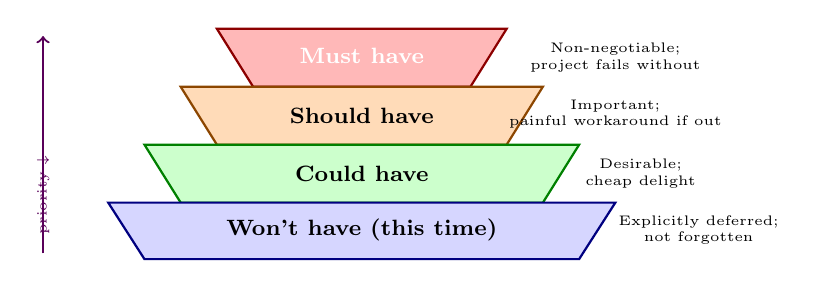
\begin{tikzpicture}[every node/.style={font=\scriptsize}, scale=0.92]
% pyramid layers with 4 colors
\draw[fill=red!28, draw=red!55!black, thick] (1.5,3.4) -- (5.5,3.4) -- (5.0,2.6) -- (2.0,2.6) -- cycle;
\node[font=\footnotesize\bfseries, white] at (3.5,3.02) {Must have};
\node[font=\tiny, align=center] at (7.0,3.0) {Non-negotiable;\\project fails without};

\draw[fill=orange!28, draw=orange!55!black, thick] (1.0,2.6) -- (6.0,2.6) -- (5.5,1.8) -- (1.5,1.8) -- cycle;
\node[font=\footnotesize\bfseries] at (3.5,2.20) {Should have};
\node[font=\tiny, align=center] at (7.0,2.22) {Important;\\painful workaround if out};

\draw[fill=green!20, draw=green!50!black, thick] (0.5,1.8) -- (6.5,1.8) -- (6.0,1.0) -- (1.0,1.0) -- cycle;
\node[font=\footnotesize\bfseries] at (3.5,1.40) {Could have};
\node[font=\tiny, align=center] at (7.35,1.40) {Desirable;\\cheap delight};

\draw[fill=blue!16, draw=blue!50!black, thick] (0.0,1.0) -- (7.0,1.0) -- (6.5,0.22) -- (0.5,0.22) -- cycle;
\node[font=\footnotesize\bfseries] at (3.5,0.62) {Won't have (this time)};
\node[font=\tiny, align=center] at (8.15,0.62) {Explicitly deferred;\\not forgotten};

% legend arrow on left
\draw[->, thick, violet!70!black] (-0.9,0.3) -- (-0.9,3.3) node[midway, left, rotate=90, font=\tiny] {priority $\downarrow$};
\end{tikzpicture}
\caption{MoSCoW pyramid: Must sets the minimum viable product; lower layers add value only after the layer above is secure. Colour intensity mirrors priority.}
\label{fig:moscow}
\end{figure}

In a semester capstone the ``Must'' set \emph{is} the minimum viable product for demo and grading. Keep it under $60\%$ of capacity; buffer absorbs estimation error. Beware anti-patterns: labelling everything Must (no prioritisation) or silently demoting Should to Could without agreement.

Rule: if a ``Must'' slips, it is a project failure, not a re-plan. ``Won't have'' is not a rejection --- it is a recorded, agreed deferral that prevents scope creep and disappointment. Re-prioritise when effort estimates or regulations change, with the product owner and key stakeholders present.

% ============================================================
\section{Requirements Validation and Traceability}
\label{sec:validation}
Writing requirements is not enough; we must check they are correct, consistent, complete, and feasible before building.

\begin{definition}[Validation vs.\ verification] \emph{Validation}: are we building the \emph{right} thing (stakeholder need)? \emph{Verification}: are we building the thing \emph{right} (meets its spec)? Requirements validation is the first line of defence against both failures.\end{definition}
\textbf{Validation checks:} reviews and walkthroughs with stakeholders, prototyping risky flows (can a student really cancel in two taps?), model checks for contradictions (``guest checkout'' vs.\ ``all orders require login''), and testability review (can we write a Then for every requirement?). Record defects and re-elicit. Use a checklist: is each requirement unambiguous, atomic, feasible, and ranked? Any ``TBD'' is a risk flagged for the next elicitation cycle.
Typical defects: ambiguity (``quick''), incompleteness (missing error case), inconsistency (two requirements demand opposite behaviours), and gold-plating (no stakeholder asked for it).

\textbf{Traceability} connects every need forward to its realisation and backward to its source. The \emph{traceability matrix} is the audit trail: Need $\to$ Requirement $\to$ Design element $\to$ Code module $\to$ Test case. When a regulation changes, follow the links to find everything that must change.

\begin{figure}[h]
\centering
\begin{tikzpicture}[font=\scriptsize, scale=0.88,
  box/.style={draw, rounded corners=3pt, minimum width=2.0cm, minimum height=0.7cm, align=center, thick},
  arr/.style={-{Stealth}, thick}]
\node[box, fill=blue!14] (need) at (0,0) {Stakeholder\\Need (N1)};
\node[box, fill=orange!16] (req) at (3.2,0) {Requirement\\FR-07 / NFR-03};
\node[box, fill=green!16] (des) at (6.4,0) {Design\\Use case / API};
\node[box, fill=violet!14] (code) at (3.2,-1.7) {Code\\module / story};
\node[box, fill=yellow!18] (test) at (6.4,-1.7) {Test\\Gherkin / unit};
% forward arrows
\draw[arr, blue!60!black] (need) -- (req) node[midway, above, font=\tiny] {elicit};
\draw[arr, blue!60!black] (req) -- (des) node[midway, above, font=\tiny] {refines};
\draw[arr, blue!60!black] (des) -- (test) node[midway, right, font=\tiny] {verifies};
\draw[arr, blue!60!black] (des) -- (code);
\draw[arr, blue!60!black] (code) -- (test);
% backward dashed trace
\draw[arr, dashed, red!60!black] (test) to[bend left=28] node[midway, below, font=\tiny, fill=white, inner sep=1pt] {traces back} (need);
\draw[arr, dashed, red!60!black] (code) to[bend right=20] (req);
\node[font=\tiny, align=center, text=gray!60!black] at (3.2,-2.65) {Every need has a test; every test has a need.\\Gaps = missing requirement or gold-plating.};
\end{tikzpicture}
\caption{Traceability flow: solid arrows build forward; dashed arrows audit backward. A complete matrix has no orphan needs and no orphan tests.}
\label{fig:traceability}
\end{figure}

Validation also checks \emph{verification}: did we build the requirement right? A prototype walkthrough catches infeasible NFRs early (``$99.99\%$ uptime on a student budget'' fails the feasible test). Formal reviews use Fagan inspection: moderator, reader, recorder, and checklist for ambiguity, measurability, and consistency.

Tooling: a simple table suffices at capstone scale (columns: Need, Req\,ID, Priority, Source, Design ref, Test ID, Status). At scale, requirements tools (Jama, Doors) automate links; at capstone a spreadsheet with filters and conditional formatting for orphans is enough. Update it when any artefact changes --- stale traces mislead more than no traces.

A well-kept matrix also supports impact analysis: if requirement FR-07 changes, the matrix instantly lists the design docs, code modules, and tests to revisit. This is why IDs must be stable --- never reuse a deleted Req\,ID.

% ============================================================
A common capstone mistake is to jump to solution sketches before stakeholders agree on the problem. Writing even a one-page vision and ten INVEST stories first saves weeks of rework when the supervisor says ``that's not what I meant''.

\section{Key Takeaways}
Requirements begin with people, not code. The grid tells you \emph{how} to engage each group; elicitation tells you \emph{how} to listen; INVEST and use cases tell you \emph{how} to write so tests can tell you whether you succeeded. Prioritise honestly with MoSCoW and keep every link traceable --- when scope or law changes, the matrix shows the blast radius.
Good requirements are not paperwork; they are shared understanding made visible and testable. Invest time here and every later phase accelerates; skimp here and every later phase pays interest.

\section{Exercises}
\label{sec:ch02-exercises}
\begin{enumerate}[label=E2.\arabic*, leftmargin=*, itemsep=0.55em]
    \item \textbf{Power--interest in practice.} For your capstone project list six stakeholders, place them on the grid in Fig.~\ref{fig:power-interest}, and for each justify its quadrant. Name one stakeholder teams usually miss and explain the cost of missing them.
    \item \textbf{Elicitation trade-offs.} A hawker says ``the app must be easy.'' Propose one interview question, one observation plan, and one survey item that together turn ``easy'' into quantified requirements. When would you \emph{not} use a workshop for this?
    \item \textbf{INVEST audit.} Rewrite: ``As a user I want the system to be better.'' into two INVEST-compliant stories with Gherkin acceptance criteria. Explain which INVEST letters the original violates.
    \item \textbf{MoSCoW negotiation.} Your backlog has 12 features but only 7 fit the semester. Classify 3 as Must, 4 as Should, 3 as Could, 2 as Won't, and write one sentence of stakeholder justification per feature. What happens if a Must is descoped?
    \item \textbf{Traceability matrix.} Construct a $4\times5$ traceability table (4 needs $\to$ 5 tests). Plant one orphan need, one orphan test, and one inconsistency; explain how each is detected and fixed during validation.
\end{enumerate}
% End of Chapter 2
